\documentclass[conference]{IEEEtran}
\IEEEoverridecommandlockouts
% The preceding line is only needed to identify funding in the first footnote. If that is unneeded, please comment it out.
\usepackage{cite}
\usepackage{amsmath,amssymb,amsfonts}
\usepackage{graphicx}
\usepackage{textcomp}
\usepackage{xcolor}
\usepackage{titlesec}
\usepackage{textcomp}
\usepackage{epsfig}
\usepackage{algpseudocode}
\usepackage{pgfplots}
\usepackage{tikz}
\pgfplotsset{width=10cm,compat=1.9}
 \usepgfplotslibrary{external}
\usepackage{amsmath}
\usepackage{mathtools}
\DeclarePairedDelimiter{\floor}{\lfloor}{\rfloor}
\usepackage[linesnumbered,ruled,vlined]{algorithm2e}
\def\BibTeX{{\rm B\kern-.05em{\sc i\kern-.025em b}\kern-.08em
    T\kern-.1667em\lower.7ex\hbox{E}\kern-.125emX}}

\usepackage[ruled,vlined]{algorithm2e}

\tikzexternalize 
\begin{document}

\title{Detailed analysis and design of the algorithm to find Longest Zig-Zag Subsequence\\

\text{\Large{DAA Assignment 5 - Group 21}}
}

\author{\IEEEauthorblockN{Divyesh Rana}
\IEEEauthorblockA{ \text{IIT2019063}}
\and
\IEEEauthorblockN{Akash Deep}
\IEEEauthorblockA{ \text{IIT2019064}}
\and
\IEEEauthorblockN{Gopal Pedada}
\IEEEauthorblockA{ \text{IIT2019065}}
}

\maketitle

\begin{abstract}
This paper contains the design and the detailed analysis of the algorithm used to solve the following problem:Find length of the longest
subsequence of given sequence such that all elements of this are
alternating.
\end{abstract}
\section{Introduction}


The longest zig-zag subsequence problem is to find length of the longest
subsequence of given sequence such that all elements of this are
alternating. A sequence is called a zig-zag sequence if the differences between successive elements strictly alternate between positive and negative. The first difference (if one exists) may be either positive or negative. A sequence with fewer than two elements is trivially a zig-zag sequence.

If a sequence $(x1,x2,\dots,xn)$ is a alternative sequence then its element satistfy one of the following relation:

$(x1<x2>x3<x4>\dots xn)$ or

$(x1>x2<x3>x4<\dots xn)$.

This report further contains -

II. Algorithmic Design

III. Algorithm Analysis

IV. Illustration

V. Experimental Study

VI. Conclusion 

\section{Algorithmic Design}

An array $Arr$ of length $n$ consists of integers is given as an input from the user. 



\subsection{longest zig-zag subsequence using sign comparision}

We will proceed by comparing the mathematical signs(negative or positive) of the difference of two consecutive elements of $Arr$. To achieve this, we will store the sign of $(Arr[i]-Arr[i-1])$ in a variable, subsequently comparing it with that of $(Arr[i+1]-Arr[i])$.If it is different, we shall increment our result. 

In short, we compare the sign of current difference with the sign of the previous difference and if it is different then we increment the result and update the sign for previous difference and return result.

For checking the sign, we shall use a simple Signum Function, which shall determine the sign of a number passed to it. That is,

\[signum(x) =  \begin{cases} 
      1 & x > 0\\
      -1 & x<0\\
      0 & x=0
   \end{cases}
\]

\subsection{longest zig-zag subsequence using dynamic programming}
This algorithm uses Dynamic Programming.

We define a two dimensional array $dp[n][2]$ such that $dp[i][0]$ contains longest zig-zag subsequence ending at index $i$ and last element is greater than its previous element and $dp[i][1]$ contains longest zig-zag subsequence ending at index $i$ and last element is smaller than its previous element, then we have following recurrence relation between them,

For all $j<i$,

\vspace 5
$dp[i][0] = max(dp[i][0],dp[j][1]+1)$ if $Arr[j]<Arr[i]$,

$dp[i][1] = max(dp[i][1],dp[j][0]+1)$ if $Arr[j]>Arr[i]$

\vspace 5
Note that the minimum length of zig-zag subsequence can be $1$, so intialize all the elements of $dp[n][2]$ with $1$.

Run a loop with index $i$ from $0$ to $n$ and inside that loop, run another loop with index $j$ from $0$ to $i$ such that $j<i$ satisfies, now assign values in $dp[i][0]$ and $dp[i][1]$ as per relation shown above. Keep updating $result =  max(result,max(dp[i][0],dp[i][1]))$. Return result.

\vspace 5
\begin{algorithm}[H]
    \caption{Longest zig-zag subsequence using sign comparision}
    \KwIn{Array $Arr$ of size $n$}
    \KwOut{length of longest zig-zag subsequence}
    \SetKwInOut{KwRequire}{Require}
    \KwRequire{$n\geq 0$}
    \DontPrintSemicolon
    \SetKwFunction{FMain}{LZS}
    \SetKwProg{Fn}{Function}{:}{}

    \Fn{\FMain{$Arr$,$n$}}{ 

        \If{$n=0$}{
        \KwRet 0\;
        }
       $length\gets 1$\;
        $prevSign\gets 0$\;
        \For{$i \gets 1 $ \text{ to }$n-1$}{
            $sign \gets signum(Arr[i]-Arr[i-1])$\;
            \If{$sign!=prevSign$ \text{ and } $sign!=0$}{
                $length \gets length +1$\;
                $prevSign\gets sign$\;
            }
        }
        \KwRet length\;
    }
    
\end{algorithm}

\begin{algorithm}

    \caption{Longest zig-zag subsequence using dynamic programming}
    \KwIn{Array $Arr$ of size $n$}
    \KwOut{length of longest zig-zag subsequence}
    \SetKwInOut{KwRequire}{Require}
    \KwRequire{$n\geq 0$}
    \DontPrintSemicolon
    \SetKwFunction{FMain}{LZS}
    \SetKwProg{Fn}{Function}{:}{}

    \Fn{\FMain{$Arr$,$n$}}{ 
        
        \If{$n=0$}{
        \KwRet 0\;
        }
        $result\gets 1$\;
       \For{$i \gets 0$ \text{ to } $n-1$}{
            $dp[i][0]\gets 1$\;
            $dp[i][1]\gets 1$\;
       }
       
       \For{$i\gets 0$ \text{ to } $n-1$}{
            \For{$j\gets 0 $\text{ to } $i-1$}{
                \If{$Arr[j]<Arr[i]$}{
                    $dp[i][0] \gets max(dp[i][0],dp[j][1]+1)$\;
                }
                \If{$Arr[j]>Arr[i]$}{
                    $dp[i][1] \gets max(dp[i][1],dp[j][0]+1)$\;
                }
            }
            $result = max(result,max(dp[i][0],dp[i][1]))$\;
       }
        \KwRet result\;
        
    }
    
\end{algorithm}



\begin{algorithm}

    \caption{signum function}
    \KwIn{Integer $x$}
    \KwOut{sign}
    \SetKwInOut{KwRequire}{Require}
    
    \DontPrintSemicolon
    \SetKwFunction{FMain}{signum}
    \SetKwProg{Fn}{Function}{:}{}

    \Fn{\FMain{$x$}}{ 
        $sign\gets 0$\;
        \If{$x>0$}{$sign\gets 1$\;}
        \ElseIf{$x<0$}{
            $sign\gets -1$\;
        }
      
       
        \KwRet sign\;
        
    }
    
\end{algorithm}

\section{Algorithm Analysis}
\subsection{Time Complexity:}

\textbf{Approach 1:} 
Here, Only single traversal is required to complete the algorithm so the time complexity is $O(n)$.

The best case for this algorithm is $n=1$, so $T_{best}=O(1)$ and $T_{worst}=O(n)$.

\textbf{Approach 2:} 
Here, we assume that integer operations take O(1) time. Two loops are used, nested one into other. Therefore, time complexity of this algorithm is $O(n^2)$.

The best case for this algorithm is $n=1$, so $T_{best}=O(1)$ and $T_{worst}=O(n^2)$.



\subsection{Space Complexity}
The space complexity for both algorithms is $O(n)$.

\section{Illustration}

Suppose we are given an array $Arr$ = \{5, 0, 3, 1, 0\}

size of $Arr$ = 5.
\subsection{First Algorithm}

Initially $prevSign=0$ and $result =1$.

now when $i=1$, $0-5=-5 < 0 $ so $sign = -1$ and $sign\neq prevSign$, result++ and $prevSign=-1$.

when $i=2$, $3-0=3 > 0$ so $sign = 1$ and $sign\new prevSign$, result++ and $prevSign=1$.

when $i=3$, $1-3=-2<0$so $sign=-1$ and again $sign\neq prevSign$, result++ and $prevSign=-1$.

when $i=4$, $0-1=-1<0$so $sign=-1$ but this time $sign=prevSign$, so result does not increment and loop terminates.

The function returns $result=4$.

\subsection{Second Algorithm}
inside first for loop,

when i = 1, $dp[i][0] = 1$ and $dp[i][1] =2$.

when i = 2, $dp[i][0] = 3$ and $dp[i][1] = 2$.

when i = 3, $dp[i][0] = 3$ and $dp[i][1] = 4$.

when i = 4, $dp[i][0] = 1$ and $dp[i][1] = 4$.

clearly throught the computation, our $result$ will be $4$ and the length of longest zig-zag subsequence is also $4$.

\section{Experimental Analysis}


\textbf{Graph - 1 : } The first graph is showing Linear behaviour.

\textbf{Graph - 2 : } The second graph is showing $O(n^2)$ behaviour.

\begin{flushleft}

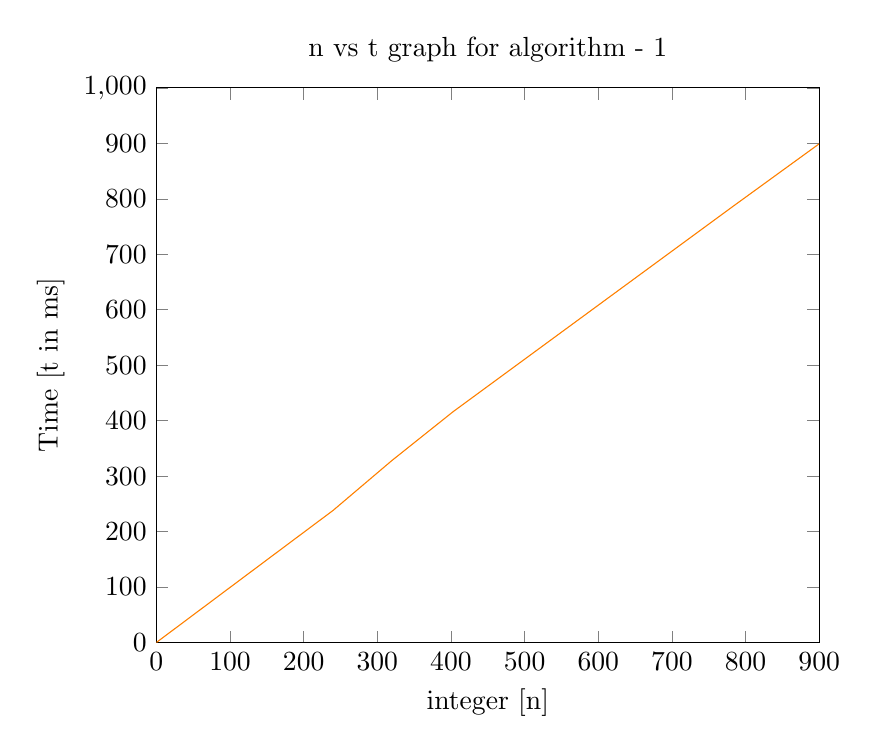
\begin{tikzpicture}

  \begin{axis}[
    title={n vs t graph for algorithm - 1},
    xlabel={integer [n]},
    ylabel={Time [t in ms]},
    xmin=0, xmax=900,
    ymin=0, ymax=1000,
    xtick={0,100,200,300,400,500,600,700,800,900},
    ytick={0,100,200,300,400,500,600,700,800,900,1000}
]
\addplot[
    color=orange,
    mark=dot,
    ]
    coordinates {
 (0,0)(100,99.3)(240,238.23)(320,328.32)(403,416.23)(783,786.45)(900,899.2)
    };
    
  \end{axis}
  


\end{tikzpicture}
\end{flushleft}


% \begin{flushleft}

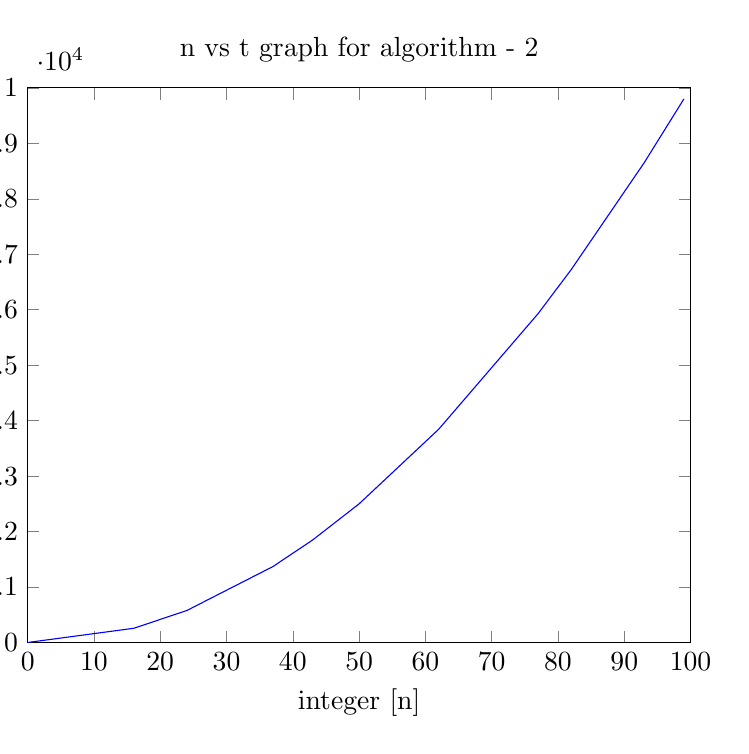
\begin{tikzpicture}[trim left=0cm]
\begin{axis}[
    title={n vs t graph for algorithm - 2},
    xlabel={integer [n]},
    ylabel={Time [t in ms]},
    xmin=0, xmax=100,
    ymin=0, ymax=10000,
    xtick={0,10,20,30,40,50,60,70,80,90,100},
    ytick={0,1000,2000,3000,4000,5000,6000,7000,8000,9000,10000}
]
\addplot[
    color=blue,
    mark=dot,
    ]
    coordinates {
  (0,0)(16,256)(24,576)(37,1369)(43,1849)(50,2500)(62,3844)(77,5929)(82,6724)(93,8649)(99,9801)
    };
    
  \end{axis}



\end{tikzpicture}
% \end{flushleft}


\section{Conclusion\\}

The second algorithm uses the dynamic programming but has the time complexity of $O(n^2)$, however first algorithm has time complexity of $O(n)$ which is better than $O(n^2)$.

\begin{thebibliography}{00}
\begin{enumerate}

    \item \url{http://www.algorithmsandme.com/longest-alternating-subsequence/}
        \item \url{https://www.geeksforgeeks.org/longest-zig-zag-subsequence/}
\end{enumerate}

\end{thebibliography}



\end{document}


% Intro by gopal, algo by Divyesh, analysis by Akash
